\clearpage
\section{Phân hệ Chi tiết Sản phẩm (Product Detail)}

\subsection{Đặc tả Use Case}
Phân hệ Chi tiết Sản phẩm cung cấp thông tin toàn diện về đồ uống, bao gồm mô tả, thành phần dinh dưỡng/nguyên liệu và cho phép khách hàng cá nhân hóa món đồ uống theo sở thích cá nhân. Sơ đồ Use Case được minh họa tại Hình~\ref{fig:usecase-product-detail}.

\begin{figure}[H]
    \centering
    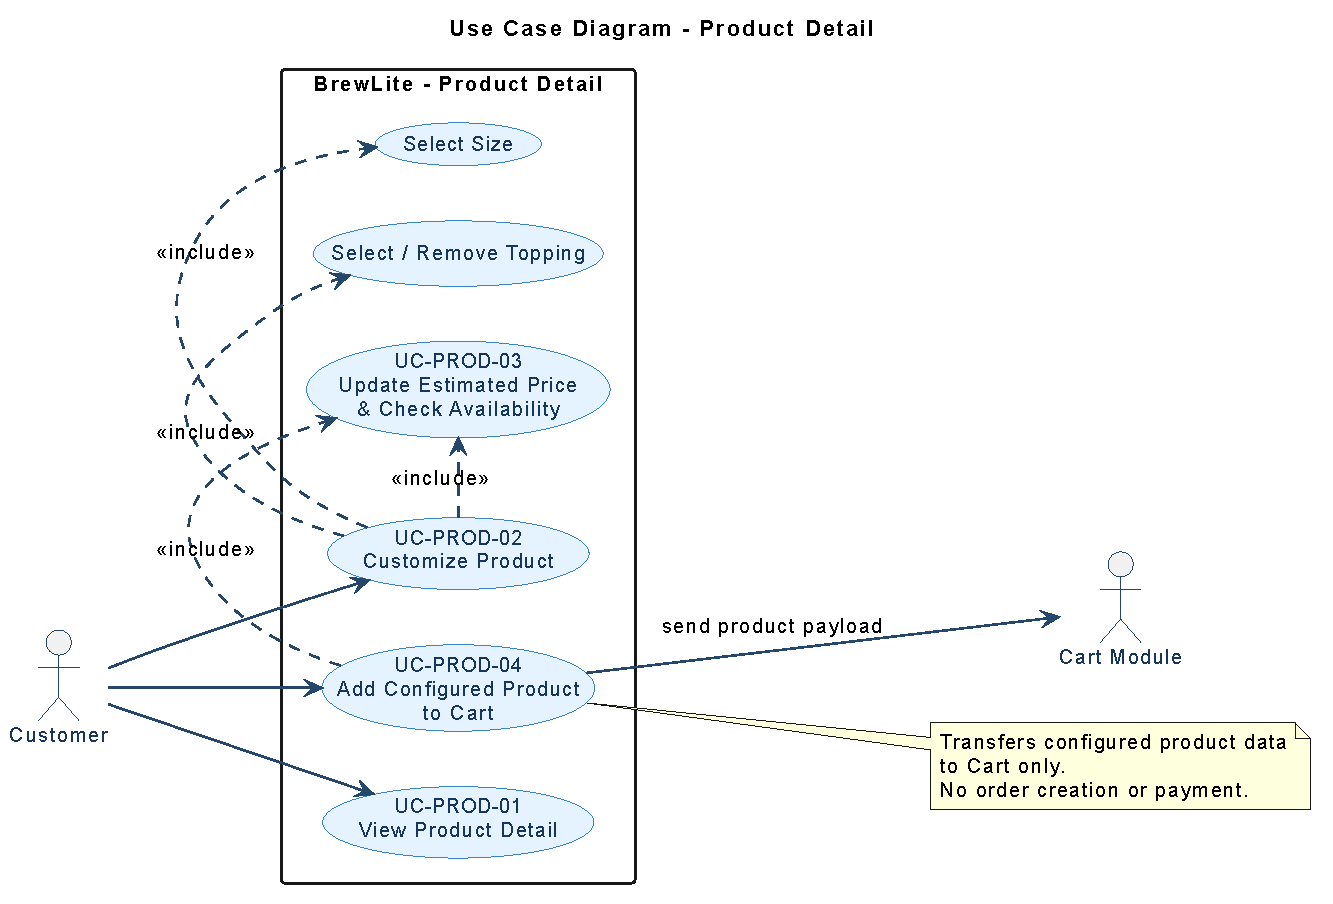
\includegraphics[width=0.75\textwidth]{figures/usecase-product-detail.pdf}
    \caption{Sơ đồ Use Case - Phân hệ Chi tiết Sản phẩm}
    \label{fig:usecase-product-detail}
\end{figure}

\begin{table}[H]
\centering
\small
\caption{Đặc tả Use Case: Xem chi tiết và Tùy biến món (UC-DET-01)}
\label{tab:uc-spec-detail}
\begin{tabularx}{\textwidth}{p{2.8cm}X}
\toprule
\textbf{Mục} & \textbf{Chi tiết Đặc tả} \\
\midrule
\textbf{Actor} & Khách vãng lai, Khách hàng đăng nhập \\
\midrule
\textbf{Tiền điều kiện} & Sản phẩm tồn tại trên hệ thống và có trạng thái \texttt{is\_available = true}. \\
\midrule
\textbf{Hậu điều kiện} & Thông tin món, các lựa chọn kích cỡ, mức ngọt, mức đá, danh sách topping và đơn giá tính toán động hiển thị đầy đủ trên màn hình. \\
\midrule
\textbf{Luồng chính} & 
1. Khách hàng nhấp vào thẻ món tại trang thực đơn.\newline
2. Trình duyệt điều hướng sang \texttt{/products/[id]}.\newline
3. Frontend gọi đồng thời \texttt{GET /api/v1/products/:id} và \texttt{GET /api/v1/toppings}.\newline
4. Giao diện hiển thị: tên món, hình ảnh, nút "Quay lại thực đơn", lựa chọn Size (Mặc định: M), mức đường (0\%, 30\%, 50\%, 70\%, 100\%), mức đá (0\%, 30\%, 50\%, 70\%, 100\%) và danh sách Topping kèm giá phụ thu.\newline
5. Khi người dùng thay đổi kích cỡ hoặc chọn thêm topping, giao diện tự động tính lại tổng đơn giá của món ăn theo thời gian thực.\newline
6. Khách hàng nhấn "Thêm vào giỏ hàng" để lưu món vào giỏ. \\
\midrule
\textbf{Luồng ngoại lệ} & 
- Sản phẩm không tồn tại: API trả về mã lỗi \texttt{404 Not Found}, giao diện hiển thị thông báo sản phẩm không tìm thấy và nút quay về thực đơn.\newline
- Sản phẩm hết hàng (\texttt{stock = 0}): Nút "Thêm vào giỏ hàng" bị vô hiệu hóa (\texttt{disabled}). \\
\bottomrule
\end{tabularx}
\end{table}

\clearpage
\subsection{Sơ đồ Hoạt động (Activity Diagram)}
Quy trình người dùng tương tác, chọn lựa tùy biến và kiểm tra trạng thái tồn kho được biểu diễn tại Hình~\ref{fig:activity-product-detail}.

\begin{figure}[H]
    \centering
    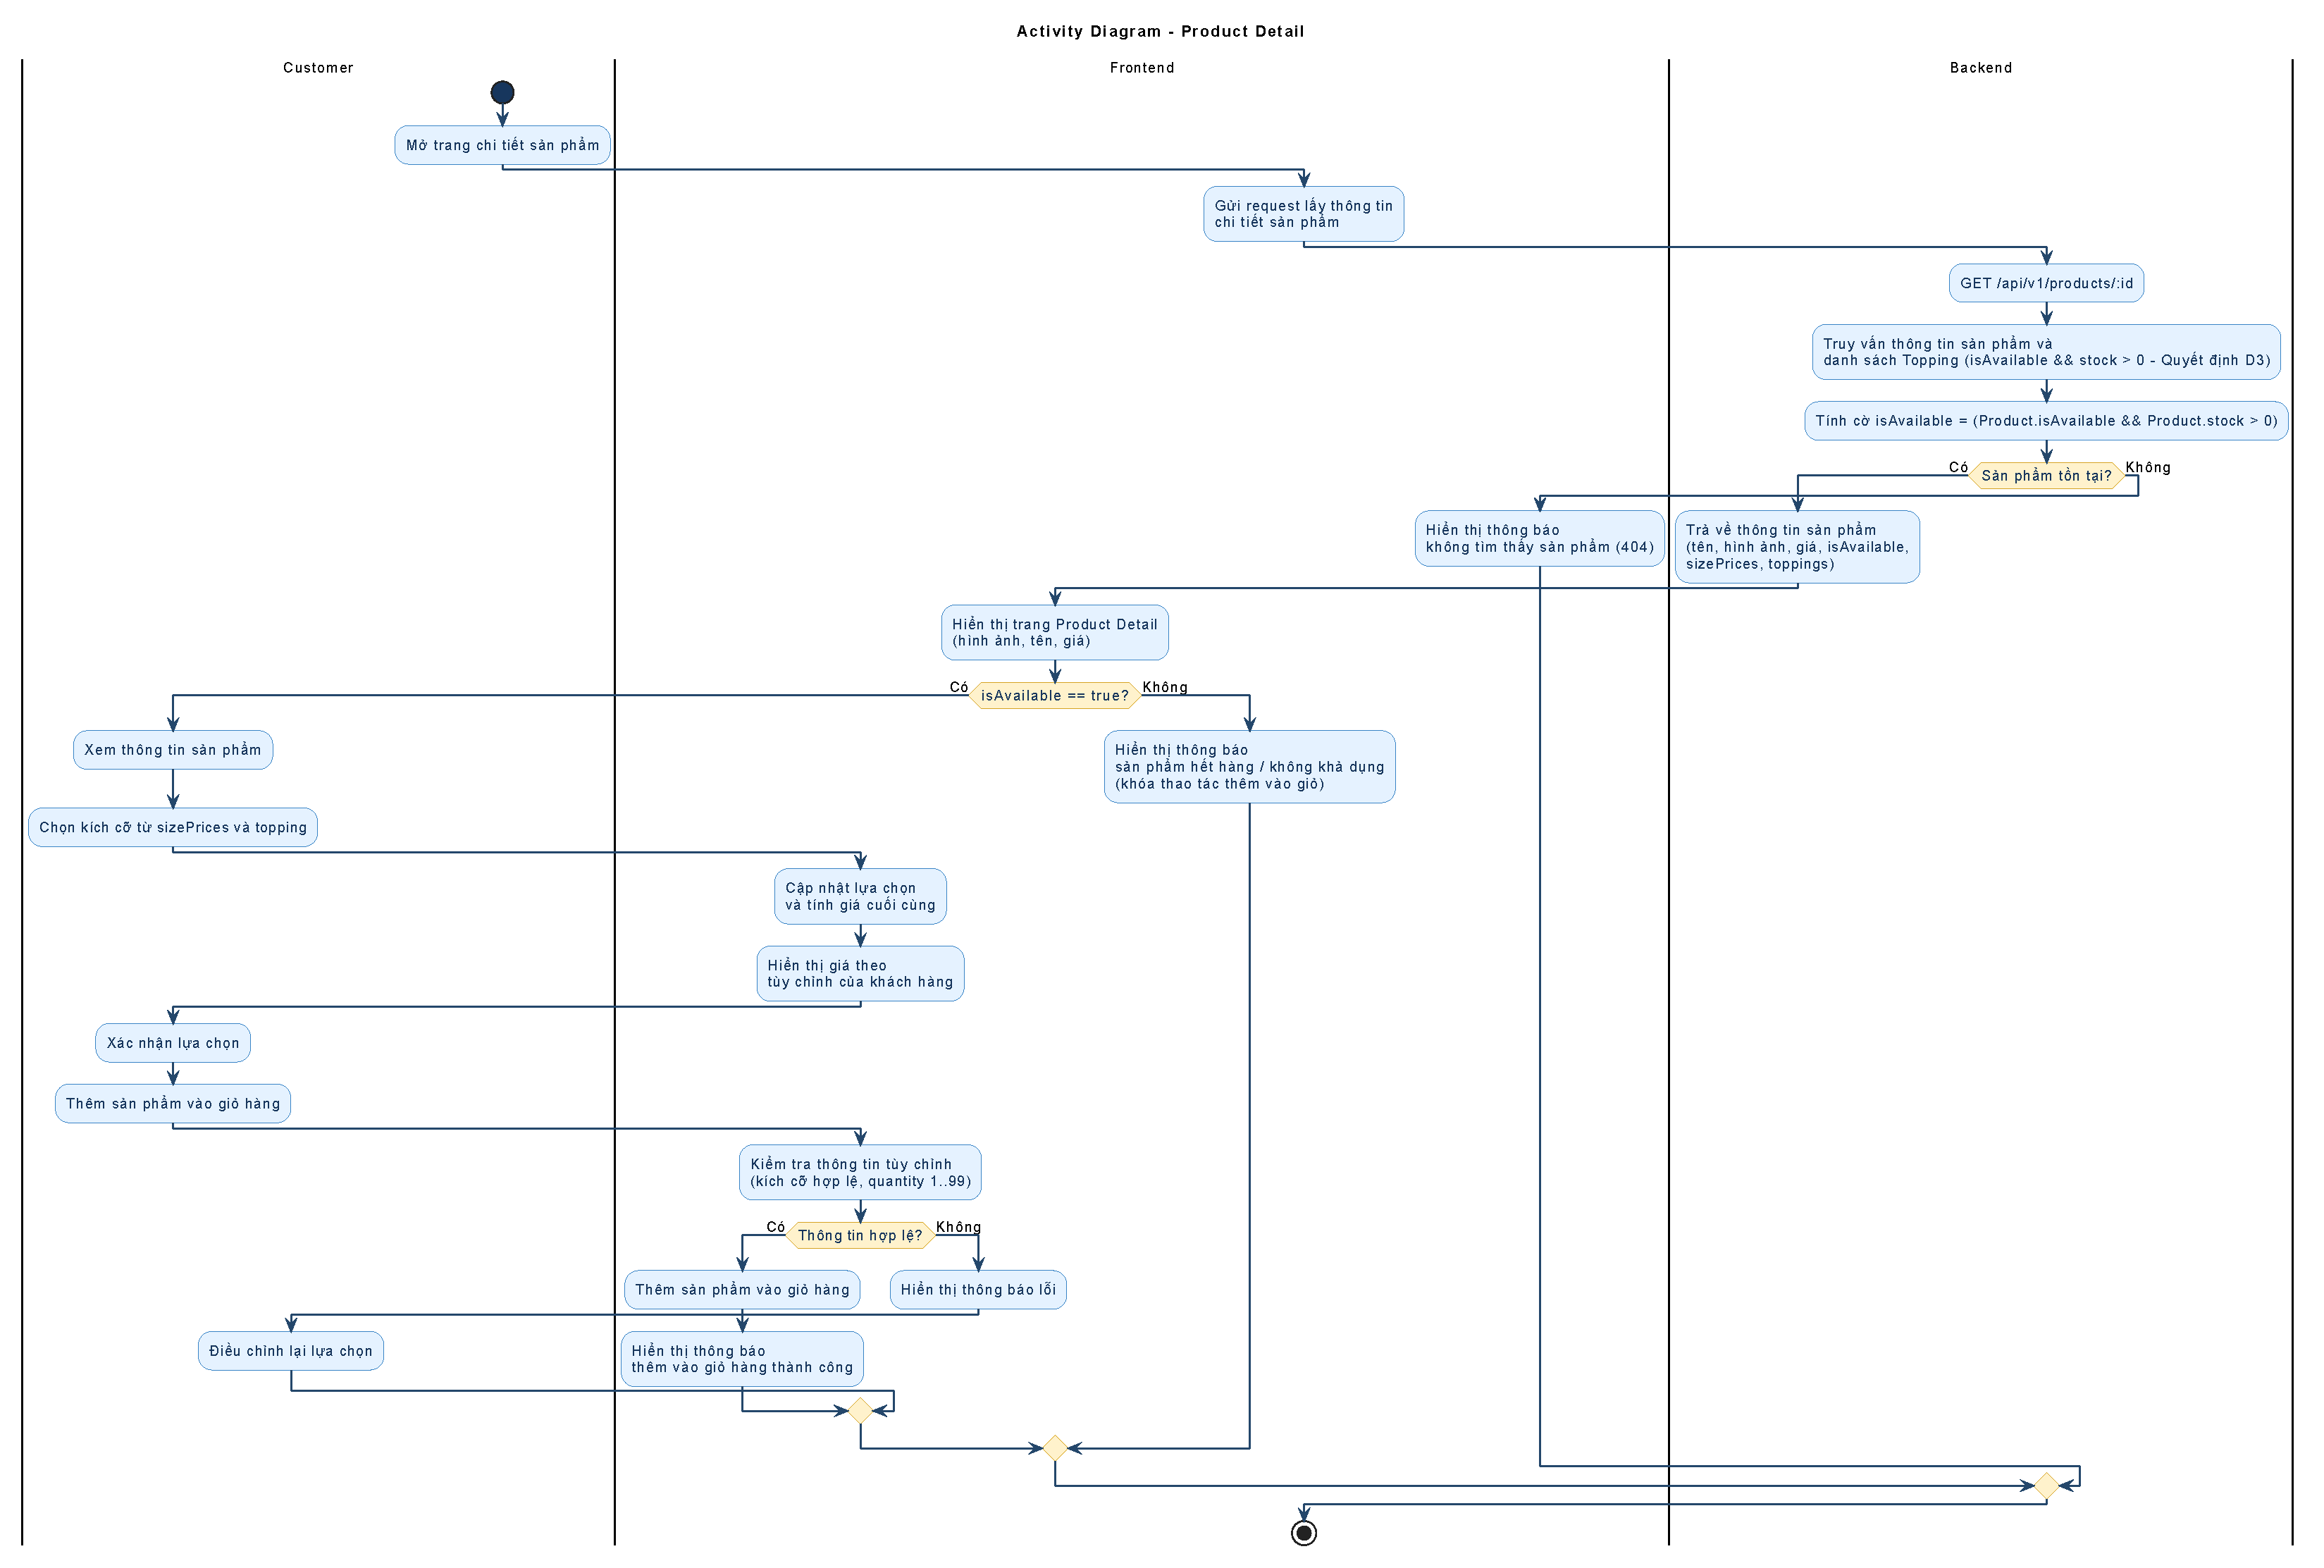
\includegraphics[width=\textwidth, height=0.80\textheight, keepaspectratio]{figures/activity-product-detail.pdf}
    \caption{Sơ đồ Hoạt động - Phân hệ Chi tiết Sản phẩm}
    \label{fig:activity-product-detail}
\end{figure}

\clearpage
\subsection{Sơ đồ Tuần tự (Sequence Diagram)}
Sơ đồ Tuần tự thể hiện các tương tác truy vấn dữ liệu chi tiết sản phẩm và danh mục topping tại Hình~\ref{fig:sequence-product-detail}.

\begin{figure}[H]
    \centering
    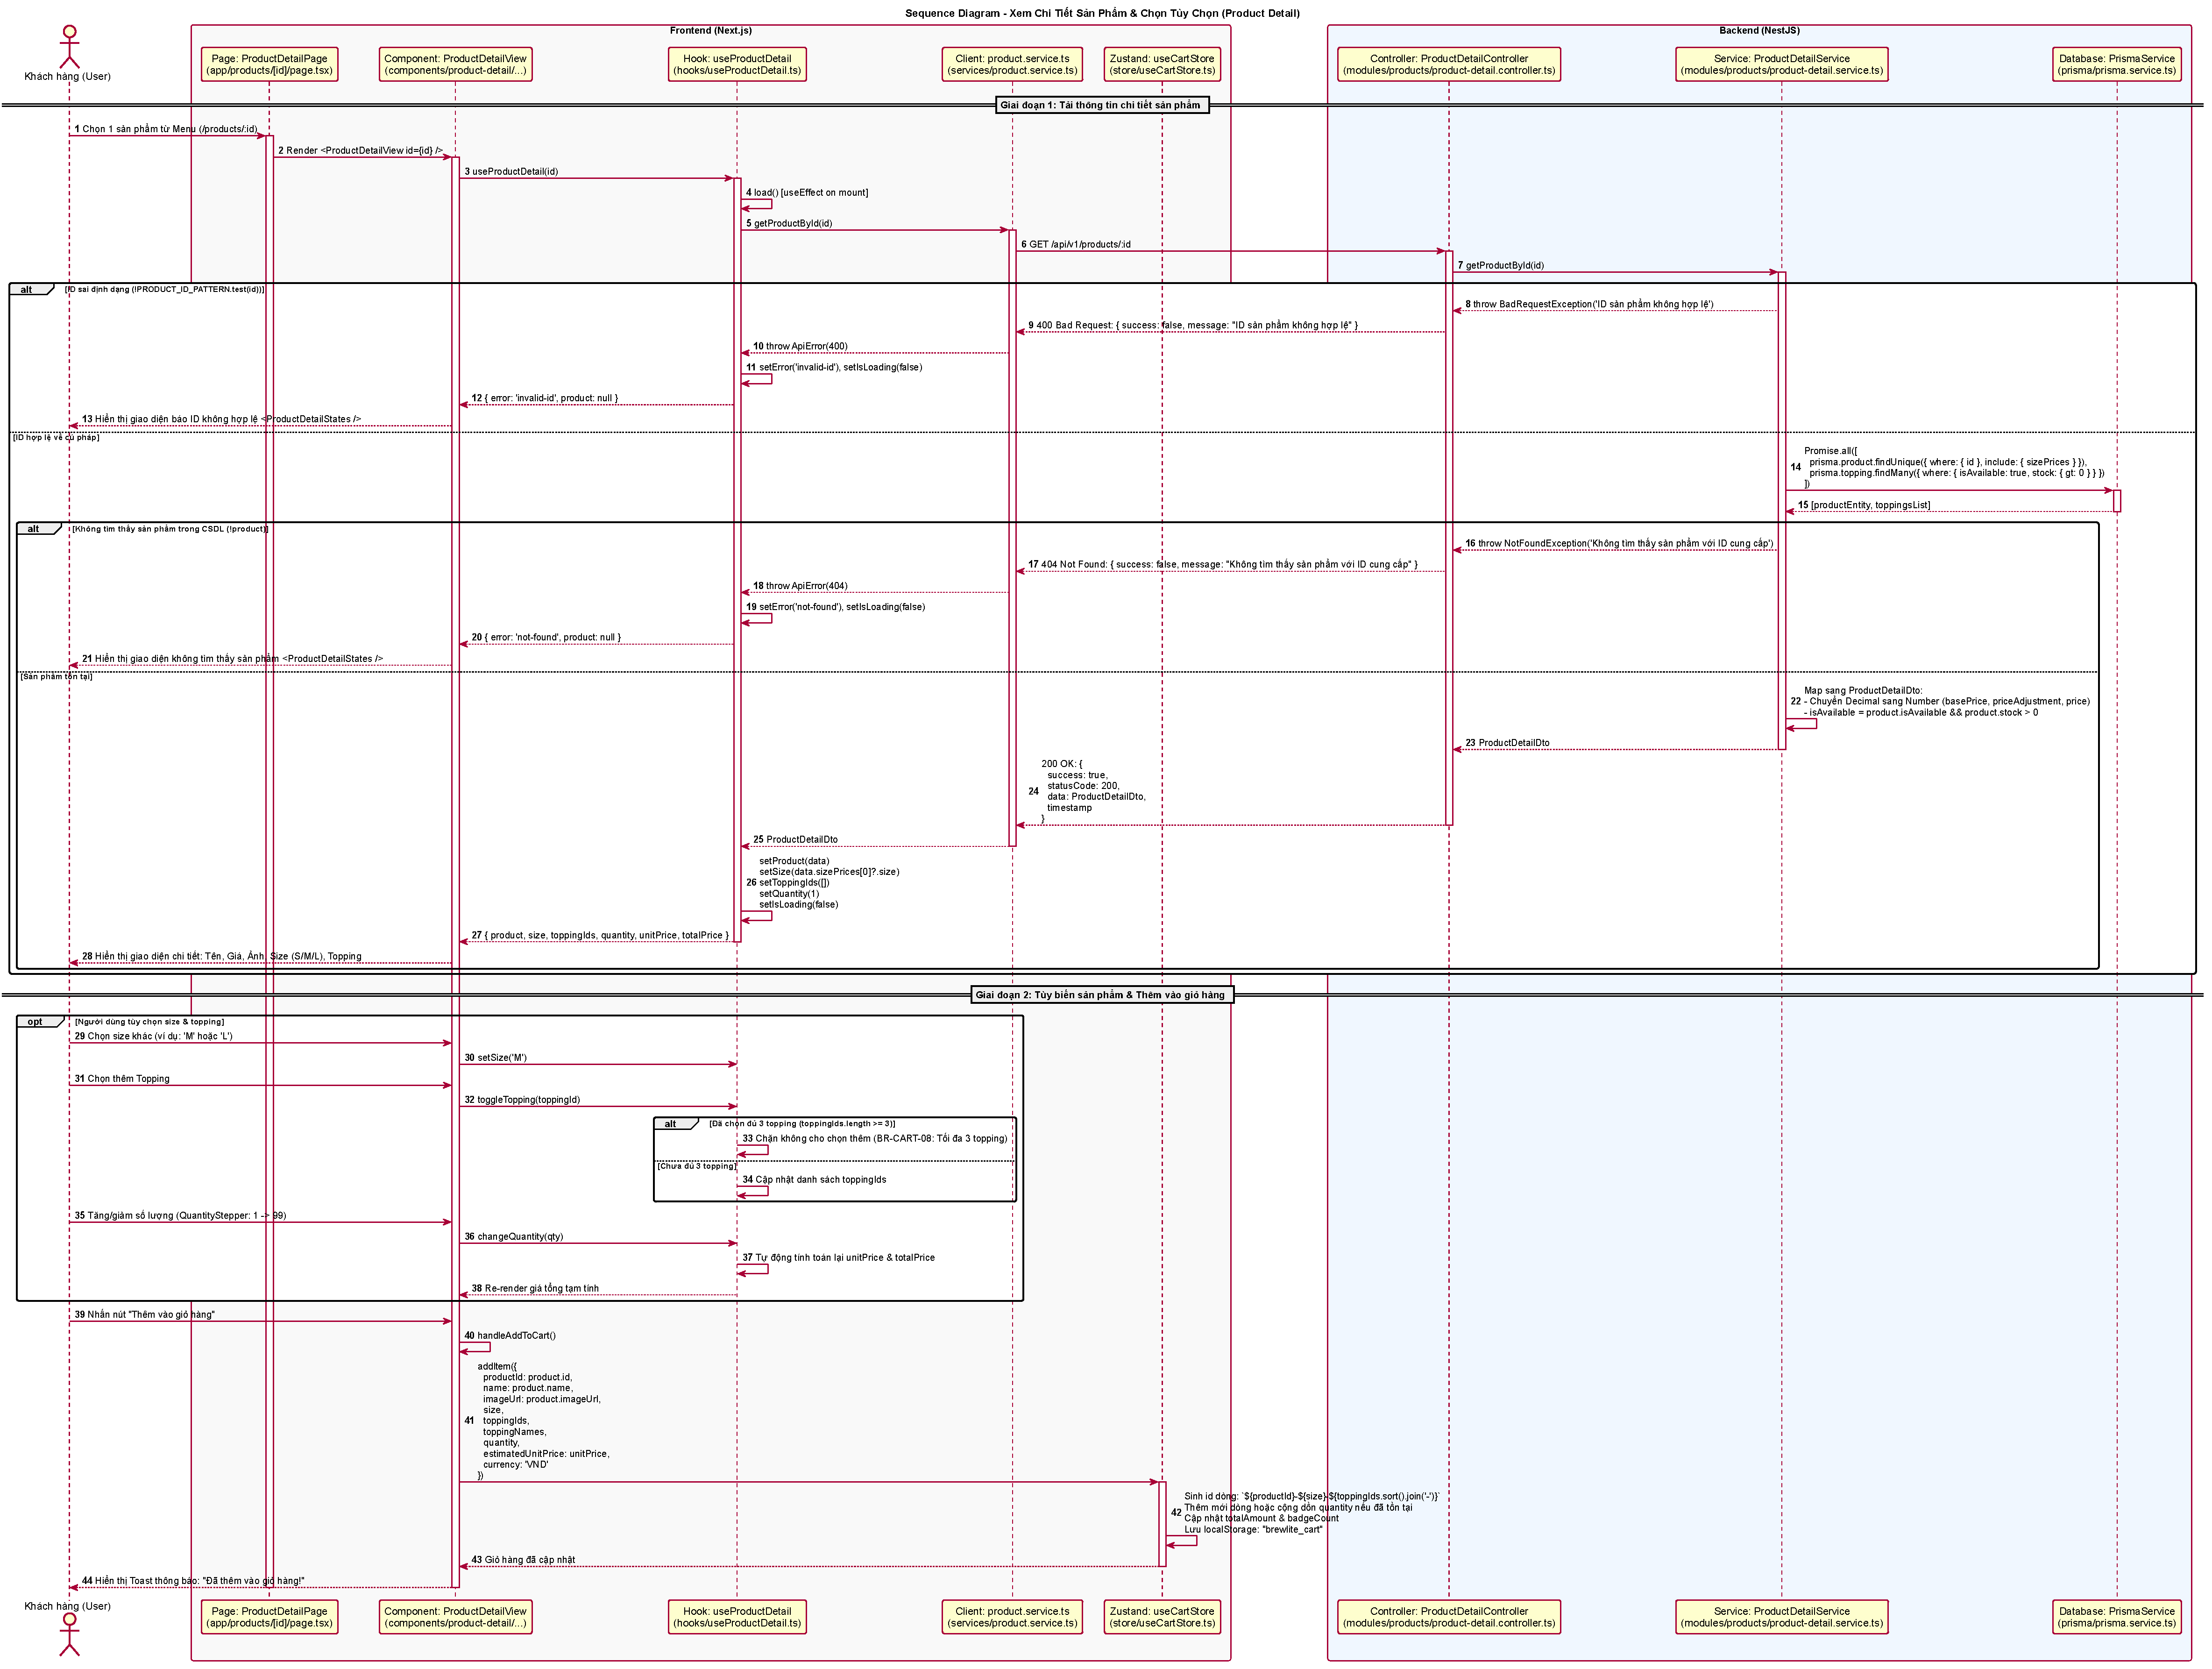
\includegraphics[width=\textwidth, height=0.80\textheight, keepaspectratio]{figures/sequence-product-detail.pdf}
    \caption{Sơ đồ Tuần tự - Phân hệ Chi tiết Sản phẩm}
    \label{fig:sequence-product-detail}
\end{figure}

\clearpage
\subsection{Hợp đồng API (API Contract)}
\begin{table}[H]
\centering
\small
\caption{Danh mục API Endpoints - Phân hệ Chi tiết Sản phẩm}
\label{tab:api-detail}
\begin{tabularx}{\textwidth}{llp{4cm}X}
\toprule
\textbf{Phương thức} & \textbf{Endpoint} & \textbf{Tham số Đường dẫn} & \textbf{Phản hồi chính} \\
\midrule
\texttt{GET} & \texttt{/api/v1/products/:id} & \texttt{id} (CUID của sản phẩm) & \texttt{200 OK}: Chi tiết sản phẩm kèm mảng \texttt{sizePrices} và thông tin \texttt{category}. Lỗi \texttt{404} nếu không tìm thấy. \\
\texttt{GET} & \texttt{/api/v1/toppings} & Không có & \texttt{200 OK}: Danh sách các loại topping đang hoạt động kèm giá và số lượng tồn. \\
\bottomrule
\end{tabularx}
\end{table}

\subsection{Ánh xạ Cơ sở dữ liệu (Database Mapping)}
\begin{itemize}
    \item Truy vấn chi tiết sản phẩm: \texttt{prisma.product.findUnique(\{ where: \{ id \}, include: \{ sizePrices: true, category: true \} \})}.
    \item Truy vấn danh sách topping: \texttt{prisma.topping.findMany(\{ where: \{ isAvailable: true \} \})}.
\end{itemize}

\subsection{Kịch bản Kiểm thử (Test Cases)}
\begin{table}[H]
\centering
\small
\caption{Tóm lược các Ca kiểm thử tiêu biểu - Phân hệ Chi tiết Sản phẩm}
\label{tab:tc-detail}
\begin{tabularx}{\textwidth}{llp{2.6cm}p{3cm}Xc}
\toprule
\textbf{Mã TC} & \textbf{Loại} & \textbf{Tiền điều kiện} & \textbf{Endpoint / Màn hình} & \textbf{Kết quả mong đợi} & \textbf{Trạng thái} \\
\midrule
\texttt{TC-DET-API-01} & Hợp lệ & ID sản phẩm tồn tại & \texttt{GET /products/:id} & HTTP 200, trả về đủ sizePrices (S, M, L) & Chưa chạy \\
\texttt{TC-DET-API-03} & Lỗi & ID không tồn tại & \texttt{GET /products/:id} & HTTP 404, message "Không tìm thấy sản phẩm" & Chưa chạy \\
\texttt{TC-DET-UI-01} & Giao diện & Mở trang chi tiết & Màn hình \texttt{/products/[id]} & Có nút "Quay lại thực đơn", nút "Thêm vào giỏ hàng" & Chưa chạy \\
\texttt{TC-DET-UI-04} & Giao diện & Chọn Size L (+10.000đ) & Tùy biến món & Đơn giá tự động cộng thêm phụ thu tương ứng & Chưa chạy \\
\bottomrule
\end{tabularx}
\end{table}

\subsection{Giao diện Người dùng}
\begin{figure}[H]
    \centering
    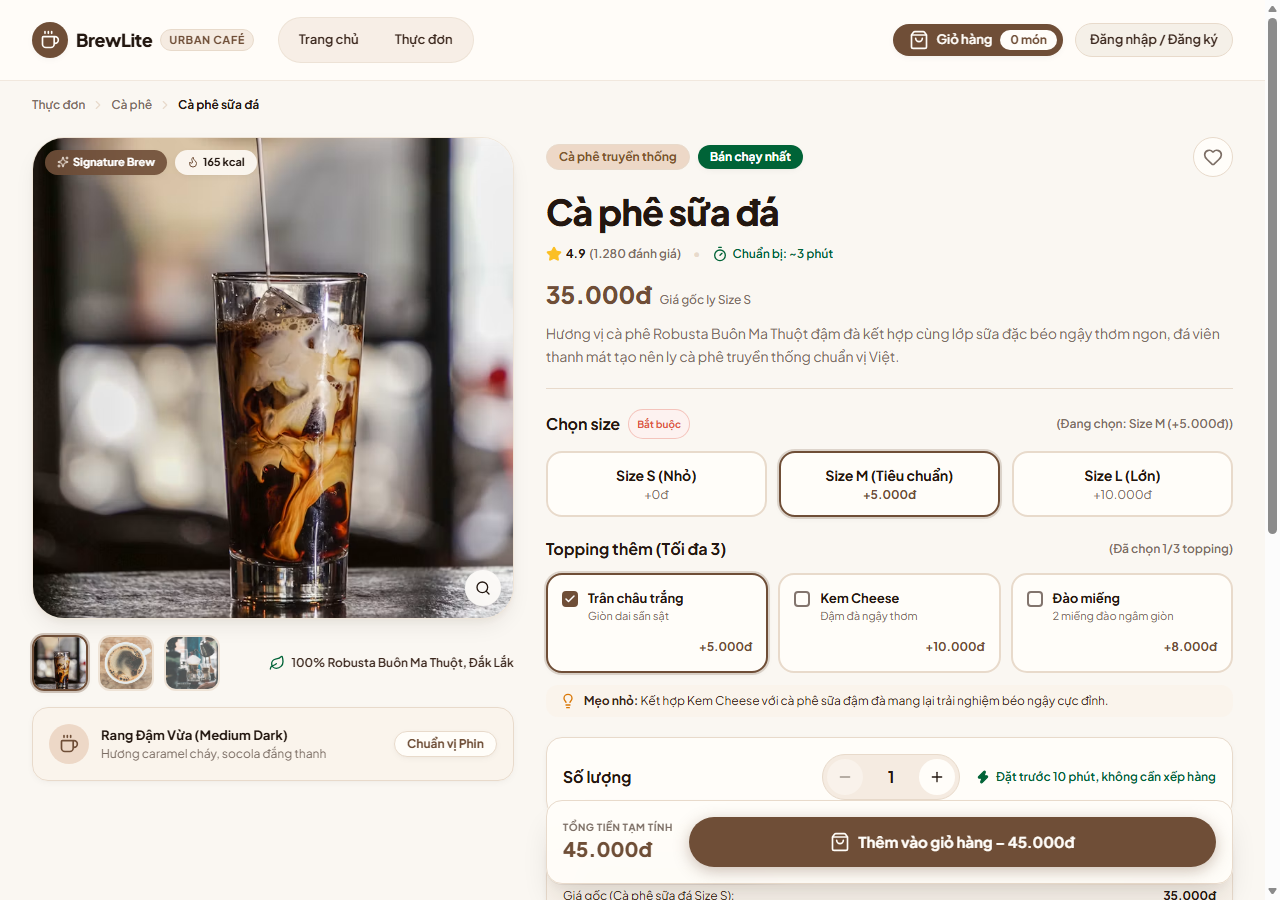
\includegraphics[width=0.92\textwidth]{figures/ui-detail.png}
    \caption{Giao diện Chi tiết món và Tùy biến Size / Topping}
    \label{fig:ui-detail}
\end{figure}
